\chapter{Grundlagen}
Dieses Kapitel befasst sich mit sowohl den mathematischen als auch den technischen Grundlagen der zu behandelnden Thematik, welche für das weitere Verständnis der Arbeit beitragen.
% -------------------------------------------------
% TECHNISCHE GRUNDLAGEN
% -------------------------------------------------
\section{Technische Grundlagen}
Im folgenden Abschnitt werden Funktionsweise und Besonderheiten der verwendeten Technologien beschrieben. Es wird eine Smartphone Anwendung erstellt, deren Grundlage für die Implementierung die Software-Plattform Android ist.
% ANDROID
\subsection{Android}


% SQLite
\subsection{Die Datenbank SQLite}
% MOBILE SENSING
\subsection{Mobile Sensorik} 
\subsubsection{Geolokation mittels \gls{GPS}}
\subsubsection{G-Sensor}
Blabla Beschleunigungssensor...
\clearpage
% -------------------------------------------------
% MATHEMATISCHE GRUNDLAGEN
% -------------------------------------------------
\section{Berechnung der Geschwindigkeitsempfehlung}
Präsentiert das System während der Anwendung eine Geschwindigkeitsempfehlung, ist diese abhängig von der Fahrtgeschwindigkeit und vom Abstand zur Ampel. Angenommen die Progressionsgeschwindigkeit $v$ wird zum Zeitpunkt $t_{1}$ ermittelt, die \gls {LSA} schaltet zum Zeitpunt $t_{2}$ auf Rot und Abstand zur Ampel beträgt $s$, dann gilt: \\
\[ v = \frac{s}{t_{2} - t_{1}} \] \\
Die von der Berliner Verkehrsleitzentrale zur Verfügung gestellten Ampelschaltpläne und Position der angesteuerten Ampel dienen als Grundlage dieser Berechnung und sind aus der Datenbank zu holen. Die aktuelle Position des Fahrrads wird vom \gls{GPS} Sensor des \glspl{Smartphone} ermittelt und daraus der Abstand zur Ampel errechnet. Die Abbildung \ref{fig:vst} soll die Berechnungsgrundlagen veranschaulichen: 
\begin{figure}[H]  
    \centering  
    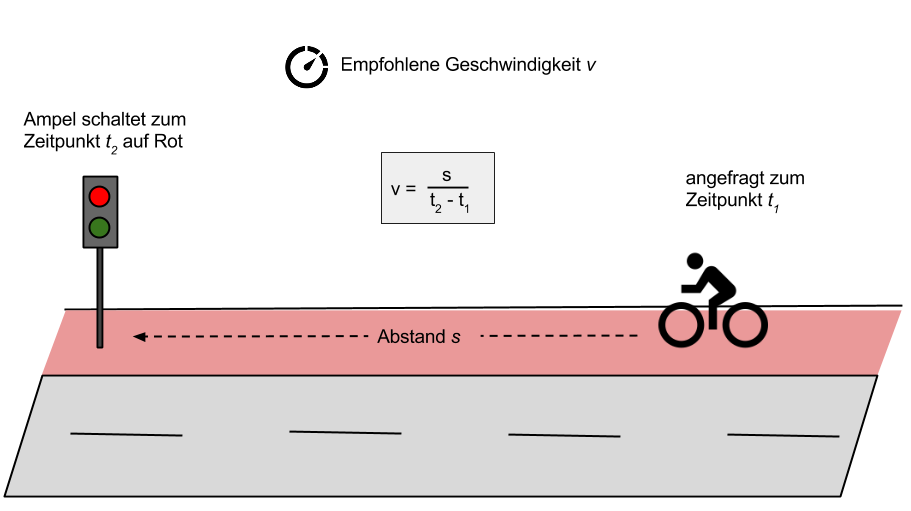
\includegraphics[width=1\textwidth]{vst}     
    \caption[Berechnung Progressionsgeschwindigkeit]{Veranschaulichung der Berechnung}
    \label{fig:vst}
\end{figure}
Um die ensprechende \gls{LSA} während der Grünphase zu passieren, muss letztendlich die empfohlene Geschwindigkeit $v$ eingehalten werden.
